\chapter{Gelombang Elektromagnetik dalam Plasma, Penghantar dan Dielektrik}\label{ch:b2:waves-in-media}

Sebuah siaran gelombang pendek menyeberangi samudra dengan memantul dari
atmosfer atas, yang memantulkannya seperti cermin --- namun lapisan yang sama
meloloskan sinyal televisi dan satelit. Sendok logam berkilau, jala
logam pada pintu oven gelombang mikro menahan gelombangnya di dalam sementara
Anda mengamati makanan Anda menembusnya, dan selembar kaca bening
bagi cahaya tetapi buram bagi ultraungu. Dalam tiap halnya sebuah gelombang memasuki
sebuah bahan, muatan bahannya menanggapi, dan tanggapannya mengubah
gelombangnya: kelajuannya, \omterm{def:b2:dispersion-wave-packets:complex}{pelemahannya}, bahkan merambat atau tidaknya
sama sekali. Bab ini menggarap ketiga model baku sebuah medium --- sebuah
gas elektron bebas, sebuah penghantar ohmik, dan elektron terikat --- dengan
satu metode yang menangani semuanya: tambahkanlah arus imbasnya pada
\omterm{thm:b2:maxwell-equations:maxwell}{persamaan Maxwell} lalu bacalah \omterm{def:b2:dispersion-wave-packets:relation}{hubungan dispersinya}.

\section{Gelombang dalam sebuah plasma}

\begin{definition}[Plasma; model elektron bebas]\label{def:b2:waves-in-media:plasma}
\index{plasma}\index{frekuensi plasma}
Yang disebut \emph{plasma} adalah gas yang netral secara keseluruhan yang terdiri atas elektron bebas (kerapatan
$n$, massa $m$, muatan $-e$) dan ion positif, yang, karena beribu-ribu
kali lebih berat, diambil sebagai tetap. Atmosfer atas (ionosfer,
$n \sim 10^{11}$--$10^{12}$ m$^{-3}$), sebuah tabung lucutan, korona matahari,
dan --- pada frekuensi optik --- elektron hantaran sebuah logam
adalah plasma. Tumbukannya diabaikan (periode gelombangnya pendek
dibandingkan waktu di antara tumbukannya). Frekuensi cirinya
adalah \emph{frekuensi plasma}
\[
\omega_p = \sqrt{\frac{ne^2}{\varepsilon_0m}} , \qquad
f_p = \frac{\omega_p}{2\pi} \approx 9\,\text{Hz}\times\sqrt{n\,[\text{m}^{-3}]} :
\]
\qty{3}{MHz} sampai \qty{9}{MHz} bagi ionosfer, \qty{2e15}{Hz} (ultraungu) bagi
sebuah logam.
\end{definition}

\begin{theorem}[Hubungan dispersi sebuah plasma]\label{thm:b2:waves-in-media:plasmadispersion}
\index{frekuensi ambang (plasma)}\index{gelombang evanesen (plasma)}
Bagi gelombang PPH transversal $\underline{\vect E} = \underline{\vect E}_0\eu^{\iu(\omega t - kx)}$ dalam
sebuah \omterm{def:b2:waves-in-media:plasma}{plasma}, elektronnya berayun dengan $\underline{\vect v} = -e\underline{\vect E}/\iu m\omega$
lalu mengemban \omterm{def:b2:charges-currents-conduction:densities}{rapat arus} $\underline{\vect j} = \underline\gamma\underline{\vect E}$ dengan
$\underline\gamma = ne^2/\iu m\omega$; \omterm{thm:b2:maxwell-equations:maxwell}{persamaan Maxwell} lalu memberi
\[
k^2 = \frac{\omega^2 - \omega_p^2}{c^2} .
\]
Di atas $\omega_p$ gelombangnya merambat, dengan $v_\varphi = c/\sqrt{1 - \omega_p^2/\omega^2}
> c$ dan $v_g = c\sqrt{1 - \omega_p^2/\omega^2} < c$, $v_\varphi v_g = c^2$; di bawah
$\omega_p$, $k = -\iu\kappa$ dengan $\kappa = \sqrt{\omega_p^2 - \omega^2}/c$: gelombangnya bersifat
\emph{evanesen}, menembus sepanjang $1/\kappa$ dan terpantul seluruhnya
(\cref{ch:b2:wave-interfaces}); \omterm{def:b2:waves-in-media:plasma}{plasmanya} lalu menjadi cermin. Pada $\omega
\gg \omega_p$ elektronnya tak sanggup mengikuti dan \omterm{def:b2:waves-in-media:plasma}{plasmanya} menjadi bening.
\end{theorem}

\begin{proof}
Persamaan geraknya $m\,\dd\vect v/\dd t = -e\vect E$ (gaya magnetiknya
$ev B \sim evE/c$ dapat diabaikan bagi $v \ll c$, dan gerak ionnya
$m/M$ kali lebih kecil): $\iu m\omega\underline{\vect v} = -e\underline{\vect E}$. Lalu
$\underline{\vect j} = -ne\underline{\vect v}$. \omterm{def:b2:waves-in-media:plasma}{Plasmanya} tetap netral bagi
gelombang transversal ($\vect k\cdot\vect E = 0$ memberi $\rho = 0$ lewat Gauss), jadi
Maxwell--Ampère berbunyi $-\iu\vect k\wedge\underline{\vect B} = \mu_0\underline\gamma\underline{\vect E}
+ \iu\omega\mu_0\varepsilon_0\underline{\vect E}$ dan Maxwell--Faraday $\underline{\vect B} = \vect k
\wedge\underline{\vect E}/\omega$; digabungkan, $k^2\underline{\vect E} = \mu_0(\iu\omega\underline\gamma -
\omega^2\varepsilon_0)(-1)\underline{\vect E}$, yakni $k^2 = \omega^2\mu_0\varepsilon_0 - \iu\omega\mu_0
\underline\gamma = (\omega^2 - ne^2/\varepsilon_0m)/c^2$. Kecepatannya menyusul seperti dalam
\cref{ch:b2:dispersion-wave-packets}.
\end{proof}

\begin{remark}[Ke mana energinya pergi]\label{rem:b2:waves-in-media:plasmaenergy}
Konduktivitasnya khayal: $\langle\vect j\cdot\vect E\rangle = 0$,
elektronnya mengambil energi dari gelombangnya selama separuh daur lalu mengembalikannya
selama separuh berikutnya --- sebuah medium tanpa rugi, yang di dalamnya energi gelombangnya
terbagi antara medannya dan energi kinetik elektronnya, dan
berjalan dengan $v_g$. Tumbukan menambahkan bagian nyata yang kecil pada $\underline\gamma$ dan
serapan yang kecil: lapisan D ionosfer menyerap gelombang menengah pada
siang hari, itulah sebabnya pemancar gelombang menengah yang jauh tertangkap pada malam hari.
\end{remark}

\begin{example}[Ionosfer dan radio]\label{ex:b2:waves-in-media:ionosphere}
Dengan $n = \qty{1e12}{m^{-3}}$ dalam lapisan F, $f_p = \qty{9}{MHz}$: siaran
gelombang pendek di bawah nilai itu terpantul (dan dapat melompat mengelilingi Bumi
antara ionosfer dan tanahnya), FM (\qty{100}{MHz}), televisi
dan sambungan satelit lolos. Gelombang \qty{3}{MHz} hanya menembus
$1/\kappa = c/\sqrt{\omega_p^2 - \omega^2} = \qty{6}{m}$ ke dalam lapisannya sebelum
berbalik. Sebuah wahana yang masuk kembali ke atmosfer terselubungi
\omterm{def:b2:waves-in-media:plasma}{plasma} dengan $n \sim 10^{18}$ m$^{-3}$, $f_p \sim \qty{10}{GHz}$: hubungan radionya
terputus bermenit-menit.
\end{example}

\begin{omfigure}
\begin{tikzpicture}
\begin{axis}[omaxis, axis x line=bottom, axis y line=left, width=6.2cm, height=4.6cm,
    xlabel={$kc/\omega_p$}, ylabel={$\omega/\omega_p$}, xmin=0, xmax=3, ymin=0, ymax=3.3, xtick={1,2,3}, ytick={1,2,3}, samples=80,
    xlabel style={at={(axis description cs:0.5,-0.12)}, anchor=north},
    ylabel style={at={(axis description cs:-0.12,0.5)}, rotate=90, anchor=south},
    legend style={font=\scriptsize, at={(0.97,0.05)}, anchor=south east, draw=none, fill=none}]
  \addplot[omThm, thick, domain=0:3] {sqrt(1+x*x)};
  \addplot[omDef, dashed, domain=0:3] {x};
  \addplot[black, dotted] coordinates {(0,1) (3,1)};
  \legend{plasma, $\omega = ck$}
  \node[font=\scriptsize, anchor=west] at (axis cs:0.1,0.5) {evanesen};
\end{axis}
\end{tikzpicture}
\hfill
\begin{tikzpicture}[font=\small, x=1cm, y=1cm, >=Stealth]
  \draw[thick] (-3.4,0) -- (3.4,0); \node[font=\footnotesize] at (2.9,-0.3) {tanah};
  \draw[omExo, thick, dashed] (-3.4,2.6) -- (3.4,2.6); \node[omExo, font=\footnotesize] at (2.6,2.85) {ionosfer, $n_e$};
  \draw[omThm, thick, ->] (-3.0,0) -- (-1.5,2.55); \draw[omThm, thick, ->] (-1.5,2.55) -- (0,0.0); \draw[omThm, thick, ->] (0,0) -- (1.5,2.55); \draw[omThm, thick, ->] (1.5,2.55) -- (3.0,0);
  \node[omThm, font=\footnotesize] at (-2.2,1.6) {$f < f_p$};
  \draw[omDef, thick, ->] (-1.0,0) -- (0.4,3.3) node[right, font=\footnotesize] {$f > f_p$};
\end{tikzpicture}

{\small Kiri: \omterm{def:b2:dispersion-wave-packets:relation}{hubungan dispersi} sebuah \omterm{def:b2:waves-in-media:plasma}{plasma} --- tak ada perambatan
di bawah $\omega_p$, sebuah hiperbola yang mendekati garis cahaya di atasnya. Kanan:
gelombang pendek di bawah \omterm{def:b2:waves-in-media:plasma}{frekuensi plasmanya} dipantulkan ionosfer
lalu melompat mengelilingi Bumi; frekuensi yang lebih tinggi lolos ke antariksa.}
\end{omfigure}

\section{Gelombang dalam penghantar ohmik: efek kulit}

\begin{theorem}[Efek kulit]\label{thm:b2:waves-in-media:skin}
\index{efek kulit}\index{kedalaman kulit}
Dalam penghantar ohmik ($\vect j = \gamma\vect E$, dengan $\gamma$ nyata, pada frekuensi
yang $\omega\tau \ll 1$ dan $\varepsilon_0\omega \ll \gamma$, yakni di bawah $\sim\qty{1e16}{Hz}$ bagi
tembaga) \omterm{thm:b2:maxwell-equations:maxwell}{arus pergeserannya} dapat diabaikan dan medannya menuruti
persamaan difusi $\Delta\vect E = \mu_0\gamma\,\partial_t\vect E$. Gelombang PPH yang memasuki
penghantarnya di $x = 0$ mempunyai
\[
\underline k^2 = -\iu\mu_0\gamma\omega , \qquad \underline k = \frac{1 - \iu}\delta , \qquad
\delta = \sqrt{\frac2{\mu_0\gamma\omega}} ,
\]
sehingga $\underline E = E_0\,\eu^{-x/\delta}\eu^{\iu(\omega t - x/\delta)}$: ia teredam
sepanjang \emph{\omterm{def:b2:dispersion-wave-packets:complex}{kedalaman kulit}} $\delta$, dengan fase yang juga berputar satu
radian tiap $\delta$ --- panjang gelombangnya $2\pi\delta$, \omterm{def:b2:dispersion-wave-packets:relation}{kecepatan fasenya} $\omega\delta \ll
c$. Arus $\vect j = \gamma\vect E$ terkurung dalam lapisan setebal
$\delta$ di bawah permukaannya, dan $\vect B$ tertinggal \qty{45}{\degree} dari $\vect E$ dengan
$|B| = |E|\sqrt2/\omega\delta$. Bagi tembaga, $\delta = \qty{9.2}{mm}$ pada \qty{50}{Hz},
\qty{0.21}{mm} pada \qty{100}{kHz}, \qty{2.1}{\micro m} pada \qty{1}{GHz}.
\end{theorem}

\begin{proof}
$\operatorname{\vect{curl}}\vect B = \mu_0\gamma\vect E$ (pergeserannya dibuang) dan
$\operatorname{\vect{curl}}\vect E = -\partial_t\vect B$: dengan mengambil curl yang kedua,
$-\Delta\vect E = -\mu_0\gamma\partial_t\vect E$ (penghantarnya netral, $\operatorname{div}
\vect E = 0$). Bagi $\eu^{\iu(\omega t - kx)}$: $k^2 = -\iu\mu_0\gamma\omega$, dan
$\sqrt{-\iu} = (1 - \iu)/\sqrt2$ memberi $\underline k = (1 - \iu)/\delta$ (akar yang
meluruh ke dalam penghantarnya). Faraday: $\underline B = \underline k\underline E/\omega = (1 - \iu)
\underline E/\omega\delta$, bermodulus $\sqrt2E/\omega\delta$ dan berfase $-\pi/4$.
\end{proof}

\begin{omfigure}
\begin{tikzpicture}
\begin{axis}[omaxis, axis x line=middle, axis y line=left, width=7.0cm, height=4.4cm,
    xlabel={$x/\delta$}, ylabel={$E/E_0$}, xmin=0, xmax=6, ymin=-1.1, ymax=1.15, xtick={0,2,4,6}, ytick={-1,1}, samples=200,
    xlabel style={at={(axis description cs:1.0,0.5)}, anchor=west},
    ylabel style={at={(axis description cs:-0.08,0.5)}, rotate=90, anchor=south}]
  \addplot[omThm, thick, domain=0:6] {exp(-x)*cos(deg(x))};
  \addplot[omDef, dashed, domain=0:6] {exp(-x)};
  \addplot[omDef, dashed, domain=0:6] {-exp(-x)};
\end{axis}
\end{tikzpicture}
\hfill
\begin{tikzpicture}
\begin{axis}[omaxis, axis x line=bottom, axis y line=left, width=6.4cm, height=4.4cm,
    xmode=log, ymode=log, xmin=10, xmax=1e10, ymin=1e-7, ymax=1e-1,
    xlabel={$f$ (Hz)}, ylabel={$\delta$ (m)}, xtick={1e1,1e3,1e5,1e7,1e9}, ytick={1e-6,1e-4,1e-2},
    xlabel style={at={(axis description cs:0.5,-0.12)}, anchor=north},
    ylabel style={at={(axis description cs:-0.14,0.5)}, rotate=90, anchor=south}, samples=50,
    legend style={font=\scriptsize, at={(0.97,0.95)}, anchor=north east, draw=none, fill=none}]
  \addplot[omThm, thick, domain=10:1e10] {sqrt(2/(4*pi*1e-7*6e7*2*pi*x))};
  \addplot[omDef, thick, domain=10:1e10] {sqrt(2/(4*pi*1e-7*5*2*pi*x))};
  \legend{tembaga, air laut}
\end{axis}
\end{tikzpicture}

{\small Kiri: medan di dalam sebuah penghantar --- sebuah ayunan teredam,
mati dalam beberapa \omterm{def:b2:dispersion-wave-packets:complex}{kedalaman kulit}. Kanan: \omterm{def:b2:dispersion-wave-packets:complex}{kedalaman kulit} tembaga dan
air laut terhadap frekuensi: bermilimeter pada frekuensi jala-jala,
bermikrometer pada gigahertz; lautnya hanya meloloskan gelombang radio yang terpanjang.}
\end{omfigure}

\begin{example}[Akibat efek kulit]\label{ex:b2:waves-in-media:skinuses}
\index{hambatan bolak-balik}\index{sangkar Faraday}
(i) Sebuah kawat berjari-jari $a \gg \delta$ mengemban arusnya dalam cincin
setebal $\delta$: hambatannya naik dari $1/\gamma\pi a^2$ menjadi sekitar $1/\gamma
2\pi a\delta$ tiap meter --- bagi kawat tembaga \qty{1}{mm}, empat kali nilai
searahnya pada \qty{1}{MHz}, seratus kali pada \qty{1}{GHz}. Kumparan frekuensi tinggi
memakai kawat ``Litz'' (banyak untai yang terisolasi) atau tabung bersepuh perak;
penghantar jaringan dayanya dipilin dengan selongsong aluminium. (ii) Sebuah
kotak logam melemahkan sebuah gelombang sebesar $\eu^{-d/\delta}$ tiap ketebalan $d$: sebuah
kotak aluminium \qty{1}{mm} menghalangi \qty{1}{MHz} sebesar \qty{100}{dB} tetapi \qty{50}{Hz}
nyaris tidak sama sekali --- medan magnet berfrekuensi rendah menuntut besi. (iii)
Kapal selam hanya menerima radio gelombang sangat panjang ($\delta = \qty{2.3}{m}$ pada
\qty{10}{kHz} dalam air laut); ranjau dideteksi lewat arus pusar yang diimbaskan
sebuah kumparan padanya (\cref{ch:b2:maxwell-equations}, dengan waktu difusi
$\mu_0\gamma d^2$).
\end{example}

\section{Gelombang dalam dielektrik: elektron terikat}

\begin{proposition}[Elektron terikat elastik; indeks kompleks]\label{prop:b2:waves-in-media:lorentz}
\index{dielektrik}\index{polarisasi (medium)}\index{suseptibilitas}\index{indeks kompleks}\index{model Lorentz}
Dalam sebuah isolator tiap elektron terikat pada atomnya: simpangan
$\vect r$ dari kesetimbangannya memanggil gaya pemulih $-m\omega_0^2\vect r$ dan
peredaman $-m\Gamma\,\dd\vect r/\dd t$ (energi yang dipancarkan atau diserahkan kepada
kisinya). Digerakkan gelombangnya, $m\ddot{\vect r} = -m\omega_0^2\vect r - m\Gamma\dot{\vect r}
- e\vect E$; elektron yang tersimpangkan memberi mediumnya \emph{polarisasi}
(momen dwikutub tiap satuan volume) $\vect P = -ne\vect r = \varepsilon_0\underline\chi(\omega)
\underline{\vect E}$ dengan \emph{suseptibilitas}
\[
\underline\chi(\omega) = \frac{\omega_p^2}{\omega_0^2 - \omega^2 + \iu\Gamma\omega} ,
\qquad \omega_p^2 = \frac{ne^2}{\varepsilon_0m} ,
\]
dan arus terikatnya $\vect j = \partial_t\vect P$. \omterm{thm:b2:maxwell-equations:maxwell}{Persamaan Maxwell} lalu memberi
\[
\underline k^2 = \frac{\omega^2}{c^2}\,(1 + \underline\chi) = \frac{\omega^2}{c^2}\,\underline n^2 ,
\qquad \underline n = n' - \iu n'' ,
\]
dengan $n'$ yaitu indeks biasnya (\omterm{def:b2:dispersion-wave-packets:relation}{kecepatan fasenya} $c/n'$) dan $n''$
ekstingsinya (intensitasnya meluruh sebagai $\eu^{-2n''\omega x/c}$). Jauh di bawah sebuah
resonansi ($\omega \ll \omega_0$, $\Gamma$ diabaikan), $n'^2 \approx 1 + \omega_p^2/\omega_0^2 +
\omega_p^2\omega^2/\omega_0^4$: indeksnya \emph{naik} dengan frekuensi --- dispersi
normal, hukum Cauchy $n \approx A + B/\lambda^2$ --- dan serapannya
dapat diabaikan; dekat $\omega_0$ mediumnya menyerap, dan tepat di atasnya $n'$
turun dengan $\omega$ (dispersi anomali).
\end{proposition}

\begin{proof}
Amplitudo kompleksnya: $(\omega_0^2 - \omega^2 + \iu\Gamma\omega)\underline{\vect r} = -e\underline{\vect E}
/m$; $\underline{\vect P} = -ne\underline{\vect r}$. Lalu, seperti bagi \omterm{def:b2:waves-in-media:plasma}{plasmanya}, $k^2 = \omega^2\mu_0
\varepsilon_0 - \iu\omega\mu_0\underline\gamma$ dengan $\underline{\vect j} = \iu\omega\underline{\vect P} = \iu\omega\varepsilon_0
\underline\chi\underline{\vect E}$, yakni $\underline\gamma = \iu\omega\varepsilon_0\underline\chi$: $k^2 = (\omega^2/c^2)
(1 + \underline\chi)$. (\omterm{def:b2:waves-in-media:plasma}{Plasmanya} adalah hal $\omega_0 = 0$, $\Gamma = 0$.)
Uraiannya: $1/(\omega_0^2 - \omega^2) \approx (1 + \omega^2/\omega_0^2)/\omega_0^2$.
\end{proof}

\begin{omfigure}
\begin{tikzpicture}
\begin{axis}[omaxis, axis x line=middle, axis y line=left, width=8.4cm, height=5.0cm,
    xlabel={$\omega/\omega_0$}, ylabel={}, xmin=0, xmax=2.2, ymin=-1.6, ymax=2.4, xtick={1,2}, ytick=\empty, samples=300,
    xlabel style={at={(axis description cs:1.0,0.4)}, anchor=west},
    legend style={font=\scriptsize, at={(0.97,0.95)}, anchor=north east, draw=none, fill=none}]
  \addplot[omThm, thick, domain=0:2.2] {0.5*(1-x*x)/((1-x*x)^2+0.04*x*x)};
  \addplot[omDef, thick, domain=0:2.2] {0.5*0.2*x/((1-x*x)^2+0.04*x*x)};
  \legend{$n' - 1$, $n''$}
  \node[font=\scriptsize, anchor=south] at (axis cs:0.45,0.35) {dispersi normal};
  \node[font=\scriptsize, anchor=south west] at (axis cs:1.05,-1.5) {anomali};
\end{axis}
\end{tikzpicture}

{\small Model elektron terikat (Lorentz): bagian nyata indeksnya
naik dengan frekuensi di bawah resonansinya (dispersi normal: ungu
lebih lambat daripada merah dalam kaca), bagian khayalnya memuncak pada
resonansinya (serapan), dan indeksnya turun menembus resonansinya
(dispersi anomali).}
\end{omfigure}

\begin{example}[Kaca, air, udara]\label{ex:b2:waves-in-media:dielectrics}
Kaca mempunyai resonansi elektroniknya dalam ultraungu ($\omega_0 \sim 10^{16}$
rad/s): dalam cahaya tampak ia bening dan dispersif, $n = 1.51$ pada
\qty{700}{nm}, $1.53$ pada \qty{400}{nm}, cukup bagi sebuah prisma untuk menguraikan
pelangi dan bagi pulsa sebuah serat untuk menyebar (\cref{ch:b2:dispersion-wave-packets});
dalam ultraungu ia menyerap --- Anda tak menjadi hitam di balik jendela.
Air, selain itu, mempunyai resonansi putar molekul kutubnya dekat
\qty{20}{GHz} (sebuah relaksasi Debye alih-alih garis yang tajam): ia menyerap
gelombang mikro dengan kuat, yang lalu memanaskan makanan dan membutakan radar dalam hujan,
dan mempunyai $n'' \approx 0$ dalam jendela tampak yang sempit --- yaitu jendela yang
darinya mata berevolusi. Udara, dengan $n - 1 = 2.9 \times 10^{-4}$, tetap membengkokkan
Matahari terbenam sebesar setengah derajat.
\end{example}

\begin{remark}[Satu persamaan, tiga medium]\label{rem:b2:waves-in-media:summary}
Setiap medium linear masuk ke \omterm{thm:b2:maxwell-equations:maxwell}{persamaan Maxwell} lewat arus
imbasnya $\underline{\vect j} = \underline\gamma(\omega)\underline{\vect E}$, dan \omterm{def:b2:dispersion-wave-packets:relation}{hubungan dispersinya}
selalu $\underline k^2 = \omega^2/c^2 - \iu\omega\mu_0\underline\gamma(\omega)$:
\begin{center}\small
\begin{tabular}{lll}
medium & $\underline\gamma(\omega)$ & $\underline k^2$\\ \hline
\omterm{def:b2:waves-in-media:plasma}{plasma} & $ne^2/\iu m\omega$ (khayal) & $(\omega^2 - \omega_p^2)/c^2$: ambang\\
penghantar ohmik & $\gamma$ (nyata) & $-\iu\mu_0\gamma\omega$: \omterm{thm:b2:waves-in-media:skin}{efek kulit}\\
dielektrik & $\iu\omega\varepsilon_0\underline\chi(\omega)$ & $(\omega^2/c^2)(1 + \underline\chi)$: indeks
\end{tabular}
\end{center}
Sebuah logam adalah ketiganya bergantian: ohmik di bawah \qty{1e13}{Hz}, sebuah \omterm{def:b2:waves-in-media:plasma}{plasma}
(yang memantulkan) dalam cahaya tampak, bening dalam ultraungu jauh.
\end{remark}

\begin{method}[Gelombang dalam sebuah medium]\label{met:b2:waves-in-media:method}
(1) Tuliskanlah persamaan gerak muatannya lalu dapatkanlah $\underline{\vect j} =
\underline\gamma\underline{\vect E}$. (2) Sisipkanlah ke dalam Maxwell--Ampère dengan ansatz
PPH-nya: $\underline k^2 = \omega^2/c^2 - \iu\omega\mu_0\underline\gamma$. (3) Ambillah akar
dengan $\operatorname{Im}k \le 0$ (peluruhan searah jalannya), belahlah
menjadi bagian nyata (perambatan, $v_\varphi = \omega/k'$) dan khayal (\omterm{def:b2:dispersion-wave-packets:complex}{pelemahan}).
(4) Kenalilah rezimnya dalam frekuensi --- merambat,
evanesen, menyerap --- dan frekuensi cirinya ($\omega_p$,
$1/\mu_0\gamma\delta^2$, $\omega_0$). (5) Carilah $\vect B$ dari Faraday dan, jika perlu,
fluks Poynting serta daya yang dilesapkan.
\end{method}

\section{Latihan}

\begin{exercise}[$\star$]\label{exo:b2:waves-in-media:1}
Tentukanlah \omterm{def:b2:waves-in-media:plasma}{frekuensi plasma} bagi $n = \qty{1e11}{m^{-3}}$ (ionosfer pada malam hari),
\qty{1e12}{m^{-3}} (pada siang hari), \qty{1e18}{m^{-3}} (selubung masuk kembali), \qty{8.5e28}{m^{-3}}
(tembaga), \qty{1e5}{m^{-3}} (ruang antarbintang). Bagi masing-masingnya, mana di antara
berikut yang lolos: pemancar gelombang menengah \qty{1}{MHz}, pemancar FM \qty{100}{MHz}, sinyal
GPS \qty{1.5}{GHz}, cahaya tampak?
\end{exercise}

\begin{exercise}[$\star$]\label{exo:b2:waves-in-media:2}
Tentukanlah \omterm{def:b2:dispersion-wave-packets:complex}{kedalaman kulit} tembaga ($\gamma = \qty{6.0e7}{S/m}$) pada \qty{50}{Hz}, \qty{1}{kHz},
\qty{1}{MHz}, \qty{1}{GHz}; aluminium (\qty{3.6e7}{S/m}) pada \qty{1}{MHz}; air
laut (\qty{5}{S/m}) pada \qty{10}{kHz} dan \qty{1}{GHz}; tanah basah (\qty{1e-2}{S/m})
pada \qty{1}{MHz}. Frekuensi radio mana yang mencapai kapal selam di \qty{10}{m}?
\end{exercise}

\begin{exercise}[$\star$]\label{exo:b2:waves-in-media:3}
Sebuah kaca menuruti $n = 1.50 + \qty{4.5e3}{nm^2}/\lambda^2$. Tentukanlah indeksnya pada \qty{400}{nm},
\qty{550}{nm}, \qty{700}{nm}; \omterm{def:b2:dispersion-wave-packets:relation}{kecepatan fasenya}; indeks grupnya $n_g = n -
\lambda\,\dd n/\dd\lambda$ pada \qty{550}{nm}; sebaran sudut berkas putih yang
dibiaskan pada datang \qty{45}{\degree} ke dalam kacanya.
\end{exercise}

\begin{exercise}[$\star$]\label{exo:b2:waves-in-media:4}
Sebuah gelombang \qty{5}{MHz} menjumpai lapisan dengan $n = \qty{2e11}{m^{-3}}$: terpantulkah
ia? Kedalaman tembusnya; hal yang sama pada \qty{2}{MHz}; frekuensi minimum
yang menyeberangi lapisan dengan $n = \qty{1.5e12}{m^{-3}}$. Mengapa pita gelombang pendek
``terbuka'' dan ``tertutup'' menurut jam dan daur matahari?
\end{exercise}

\begin{exercise}[$\star\star$]\label{exo:b2:waves-in-media:5}
\emph{\omterm{ex:b2:waves-in-media:skinuses}{Hambatan bolak-balik}.} Sebuah kawat tembaga berjari-jari $a = \qty{1.0}{mm}$. (a) Hambatan
searahnya tiap meter. (b) Pada \qty{1}{MHz}: $\delta$; hambatan hampirannya
tiap meter dengan arusnya terkurung dalam cincin setebal $\delta$;
nisbahnya terhadap yang searah. (c) Pada \qty{100}{MHz}. (d) Mengapa kumparan berlilitan $N$ dari
kawat ini mempunyai faktor kualitas yang berhenti membaik dengan $N$ pada frekuensi
tinggi, dan apakah kawat Litz itu?
\end{exercise}

\begin{exercise}[$\star\star$]\label{exo:b2:waves-in-media:6}
\emph{Perisaian.} Sebuah kotak aluminium ($\gamma = \qty{3.6e7}{S/m}$) setebal \qty{1.0}{mm}.
Tentukanlah \omterm{def:b2:dispersion-wave-packets:complex}{pelemahan} amplitudo medan yang menyeberangi dindingnya, dalam dB, pada
\qty{50}{Hz}, \qty{10}{kHz}, \qty{1}{MHz} (faktor $\eu^{-d/\delta}$, dengan pemantulan di
permukaannya diabaikan). Mengapa medan magnet jala-jala diperisai
dengan besi (berpermeabilitas tinggi) alih-alih tembaga?
\end{exercise}

\begin{exercise}[$\star\star$]\label{exo:b2:waves-in-media:7}
\emph{Energi dalam sebuah \omterm{def:b2:waves-in-media:plasma}{plasma}.} Bagi gelombang transversal
\cref{thm:b2:waves-in-media:plasmadispersion}: (a) amplitudo kecepatan
elektronnya dan rapat energi kinetiknya $\tfrac12nm\langle v^2\rangle$. (b)
Rapat energi listrik dan magnetik reratanya. (c) Tunjukkanlah bahwa rapat energi
totalnya adalah $\tfrac12\varepsilon_0E_0^2(1 + \dots)$ --- hitunglah kurungnya ---
dan bahwa $\langle\Pi\rangle$ dibagi dengannya sama dengan $v_g$. (d) Berapa bagian
energinya yang berada pada elektronnya pada $\omega = 2\omega_p$?
\end{exercise}

\begin{exercise}[$\star\star$]\label{exo:b2:waves-in-media:8}
\emph{Dispersi pulsar.} Pulsa radio dari sebuah pulsar menyeberangi jarak
$L$ \omterm{def:b2:waves-in-media:plasma}{plasma} antarbintang ($n \ll$ apa pun, $\omega \gg \omega_p$). (a) Tunjukkanlah
bahwa tunda grupnya adalah $t \approx (L/c)(1 + \omega_p^2/2\omega^2)$. (b) Tunda
antara tibanya pada $f_1$ dan $f_2$ adalah $\Delta t = \dfrac{e^2}{8\pi^2
\varepsilon_0mc}\,nL\Bigl(\dfrac1{f_1^2} - \dfrac1{f_2^2}\Bigr)$: hitunglah tetapannya.
(c) Sebuah pulsar pada $L = \qty{1}{kpc} = \qty{3.1e19}{m}$ menembus $n = \qty{3e4}{m^{-3}}$:
tundanya antara \qty{400}{MHz} dan \qty{1.4}{GHz}. (d) Ahli astronomi mengukur
$\Delta t$ dan mengetahui $n$: apa yang mereka peroleh? (Ukuran dispersinya, yaitu
tolok jarak baku bagi pulsar.)
\end{exercise}

\begin{exercise}[$\star\star$]\label{exo:b2:waves-in-media:9}
\emph{Sebuah garis spektrum.} Dalam gas encer ($\underline n \approx 1 + \underline\chi/2$)
\omterm{prop:b2:waves-in-media:lorentz}{model Lorentz} memberi $n'' = \tfrac12\operatorname{Im}\underline\chi$. (a) Tunjukkanlah bahwa dekat
$\omega_0$, $n'' \approx \dfrac{\omega_p^2}{4\omega_0}\,\dfrac{\Gamma/2}{(\omega_0 - \omega)^2 + \Gamma^2/4}$, sebuah
Lorentzian berlebar penuh $\Gamma$. (b) Koefisien serapannya $\alpha = 2n''\omega/c$
di pusatnya. (c) Uap natrium, $n = \qty{1e17}{m^{-3}}$, $\lambda_0 = \qty{589}{nm}$,
$\Gamma = \qty{6e7}{s^{-1}}$: $\alpha$ di pusatnya dan tebal yang menyerap
$90\%$ (abaikanlah pelebaran Doppler, yang sebenarnya melebarkan garisnya
seratus kali lipat). (d) Sketsalah $n' - 1$ menyeberangi garisnya; di manakah
dispersinya anomali?
\end{exercise}

\begin{exercise}[$\star\star\star$]\label{exo:b2:waves-in-media:10}
\emph{Pemanasan Joule dalam kulitnya.} Sebuah gelombang $E_0\eu^{\iu\omega t}$ (sepanjang $y$)
memasuki penghantar yang mengisi $x > 0$. (a) Tuliskanlah $\underline E(x, t)$ lalu simpulkanlah
$\underline B(x, t)$ (sepanjang $z$) dari Faraday. (b) \omterm{thm:b2:poynting-vector:poynting}{Vektor Poynting} rerata di
permukaannya: tunjukkanlah $\langle\Pi_x(0)\rangle = E_0^2/2\mu_0\omega\delta$. (c) Daya Joule
rerata tiap satuan luas, $\int_0^\infty\tfrac12\gamma|\underline E|^2\dd x$: tunjukkanlah bahwa ia sama dengan
(b). (d) Nyatakanlah hasilnya sebagai $\tfrac12R_sH_0^2$ dengan $H_0 = B_0/\mu_0$ yaitu
medan magnet permukaannya dan $R_s = 1/\gamma\delta$ yaitu \emph{hambatan
permukaan}; nilainya bagi tembaga pada \qty{1}{GHz}, dan rugi sebuah
rongga gelombang mikro yang dindingnya mengemban $H_0 = \qty{100}{A/m}$.
\end{exercise}

\begin{exercise}[$\star\star\star$]\label{exo:b2:waves-in-media:11}
\emph{Mengapa logam berkilau.} Perlakukanlah elektron hantaran perak ($n =
\qty{5.9e28}{m^{-3}}$) sebagai \omterm{def:b2:waves-in-media:plasma}{plasma} tanpa tumbukan pada frekuensi optik.
(a) $\omega_p$ dan panjang gelombang yang bersesuaian. (b) Pada \qty{500}{nm}: $k$
khayal --- kedalaman tembusnya; gelombangnya terpantul seluruhnya (tanpa
serapan dalam model ini): peraknya menjadi cermin. (c) Pada \qty{200}{nm}? Dari situlah
``kebeningan ultraungu'' logam alkali. (d) Perak yang sungguhan
memantulkan $95\%$, emas tampak kuning: apa yang terlewat model ini (pikirkanlah
tumbukan, dan elektron terikat yang resonansinya terletak dalam
cahaya tampak bagi emas)?
\end{exercise}

\begin{exercise}[$\star\star\star$]\label{exo:b2:waves-in-media:12}
\emph{Air dalam gelombang mikro.} Orientasi molekul kutub air
memberi suseptibilitas $\underline\chi = \chi_s/(1 + \iu\omega\tau)$ (relaksasi
Debye), $\chi_s \approx 80$, $\tau = \qty{8}{ps}$, di atas sebuah tetapan
$\chi_\infty \approx 4$. (a) Bagian nyata dan khayal $\underline\varepsilon_r = 1 + \chi_\infty
+ \underline\chi$ pada \qty{2.45}{GHz} dan pada \qty{20}{GHz}. (b) Indeks kompleksnya dan
panjang serapan $1/(2n''\omega/c)$ intensitasnya pada \qty{2.45}{GHz}: seberapa
dalam sebuah oven memasak? (c) Daya yang terserap tiap satuan volume bagi
amplitudo medan $E_0$ dalam airnya: $\tfrac12\omega\varepsilon_0\varepsilon''E_0^2$; nilainya bagi
$E_0 = \qty{2}{kV/m}$. (d) Mengapa \qty{2.45}{GHz} yang dipakai alih-alih
\qty{20}{GHz} yang serapannya maksimum?
\end{exercise}

\begin{omfigure}
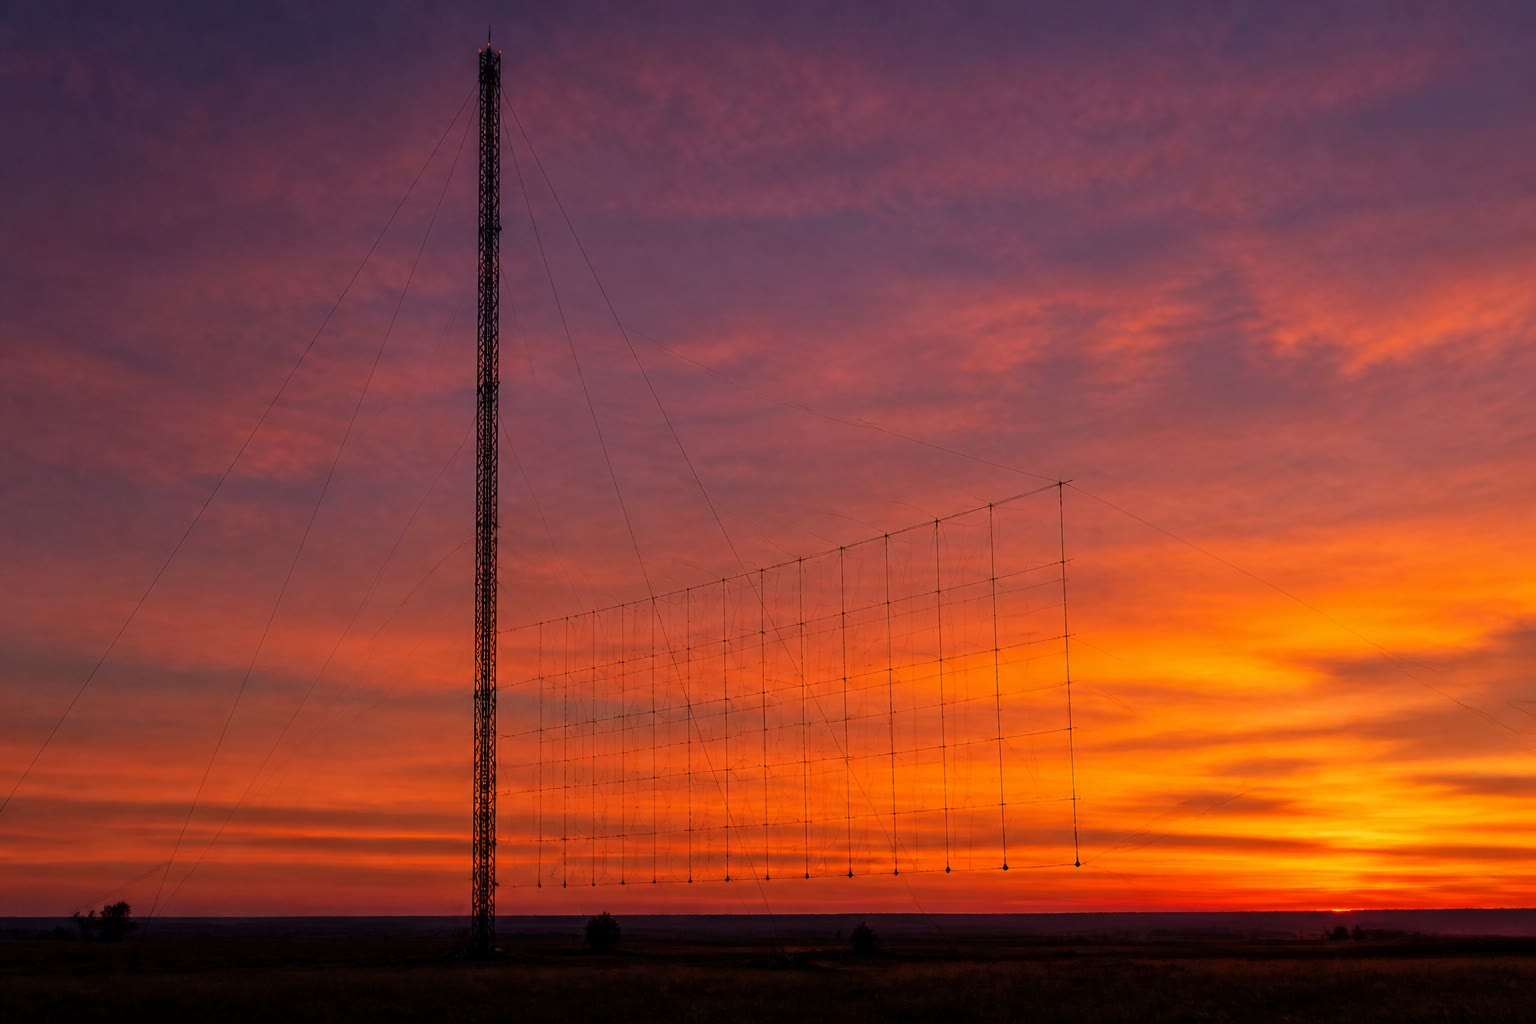
\includegraphics[width=0.58\linewidth]{images/book4/ai/b4-14-shortwave-antenna-sunset.jpg}

{\small Sebuah stasiun pemancar gelombang pendek pada senja hari: gelombangnya, beberapa megahertz di bawah \omterm{def:b2:waves-in-media:plasma}{frekuensi plasma} ionosfer, hendak dipantulkan kembali ke tanah seribu kilometer jauhnya.}
\end{omfigure}

\begin{omfigure}
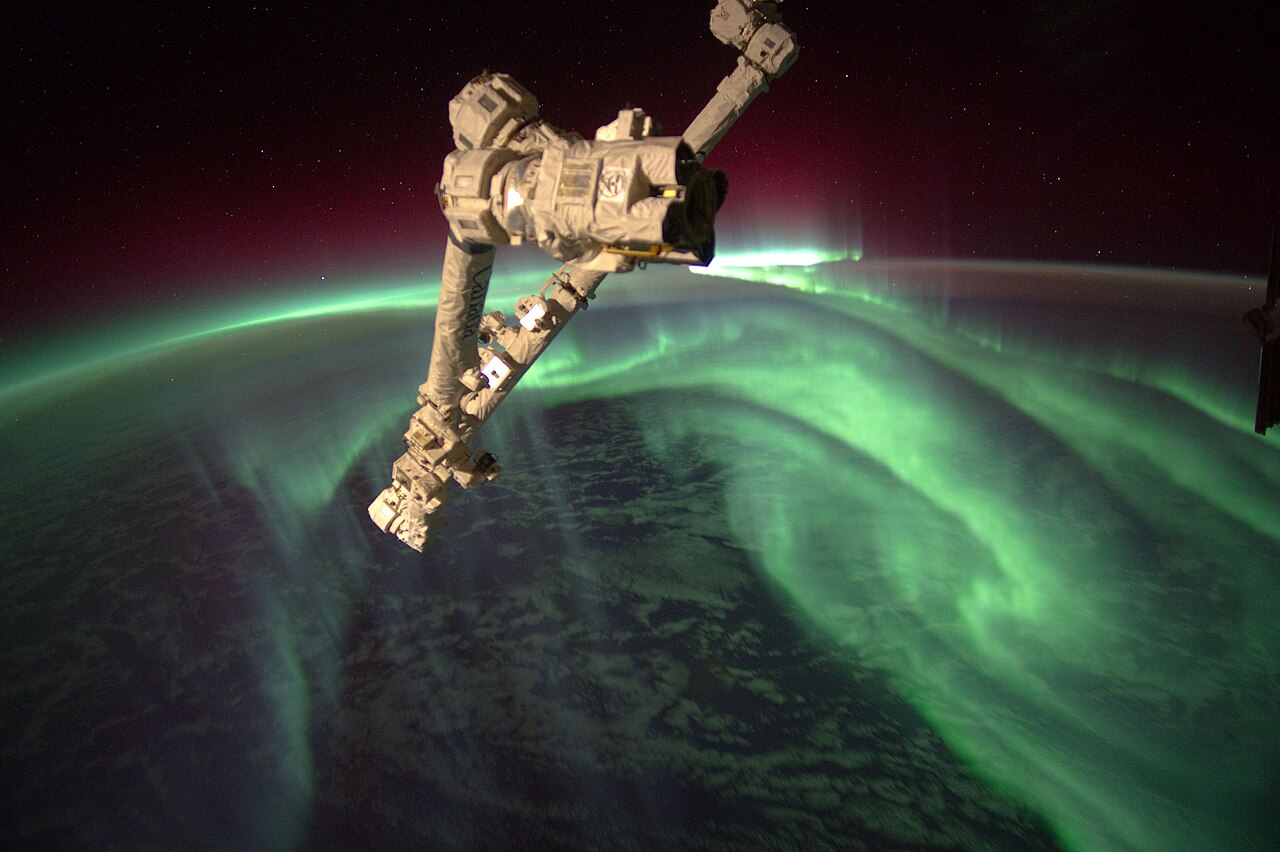
\includegraphics[width=0.6\linewidth]{images/book4/aurora-australis-iss.jpg}

{\small Aurora australis yang difoto dari Stasiun Antariksa Internasional: partikel dari Matahari, yang dipandu medan magnet Bumi, membangkitkan \omterm{def:b2:waves-in-media:plasma}{plasma} atmosfer atasnya --- yaitu ionosfer yang \omterm{def:b2:waves-in-media:plasma}{frekuensi plasmanya} memantulkan gelombang radio (NASA).}
\end{omfigure}

\section{Soal: Ionosfer, pintu oven dan prisma}

\begin{problem}[{Soal akhir pekan --- tiga bahan yang dilihat sebuah gelombang:
plasma yang membelokkan sinyal GPS, logam yang menahan gelombang mikro di dalam, dan
kaca yang menguraikan cahaya putih}]
\label{pb:b2:waves-in-media:1}

\medskip
\noindent\textbf{Bagian I --- Ionosfer dan GPS.}
Kerapatan elektron dalam lapisan F $n = \qty{1e12}{m^{-3}}$; kolom total
elektron sepanjang lintasan tegak adalah $N_T = \int n\,\dd z = \qty{2e17}{m^{-2}}$ pada
siang hari. GPS: $f_1 = \qty{1575}{MHz}$, $f_2 = \qty{1228}{MHz}$.
\begin{enumerate}
  \item \omterm{def:b2:waves-in-media:plasma}{Frekuensi plasma} lapisan F; loloskah GPS? Loloskah
        gelombang pendek \qty{5}{MHz}?
  \item Tunjukkanlah bahwa untuk $\omega \gg \omega_p$ \omterm{prop:b2:dispersion-wave-packets:group}{kecepatan grupnya} adalah $v_g \approx c(1 -
        \omega_p^2/2\omega^2)$ dan \omterm{def:b2:dispersion-wave-packets:relation}{kecepatan fasenya} $c(1 + \omega_p^2/2\omega^2)$.
  \item Tunda grup tambahan sinyal GPS yang menyeberangi lapisannya: tunjukkanlah
        $\Delta t = \dfrac{e^2}{8\pi^2\varepsilon_0mc}\,\dfrac{N_T}{f^2}$ lalu hitunglah bagi
        $f_1$; galat jaraknya $c\,\Delta t$.
  \item Penerimanya memakai kedua frekuensinya: dari kedua tundanya ia
        menyingkirkan galatnya. Nyatakanlah $N_T$ dalam $\Delta t_1 - \Delta t_2$;
        ketelitian berapa pada beda tundanya yang memberi $N_T$ sampai $1\%$?
  \item Berapa daur pembawa tambahan yang diwakili tunda pertanyaan 3
        pada $f_1$?
  \item Fase pembawanya \emph{dimajukan} sebanyak yang grupnya
        ditunda: mengapa (tanda kedua koreksinya)? Yang mana yang
        berarti bagi penerima yang mencacah daur pembawanya?
  \item Pada malam hari $N_T$ turun sepuluh kali: galat bagi penerima
        berfrekuensi tunggal pada siang dan pada malam hari.
  \item Sebuah suar matahari menaikkan $n$ dalam lapisan D (\qty{80}{km}) menjadi
        \qty{1e10}{m^{-3}} dengan banyak tumbukan: layanan radio mana yang
        terpukul, dan mengapa GPS hanya sedikit memburuk?
\end{enumerate}

\medskip
\noindent\textbf{Bagian II --- Pintu ovennya.}
Dinding rongganya dan jala pintunya terbuat dari baja ($\gamma = \qty{1.0e6}{S/m}$);
lubang jalanya selebar \qty{1.0}{mm} pada lembaran setebal \qty{0.5}{mm};
$f = \qty{2.45}{GHz}$, $P = \qty{800}{W}$.
\begin{enumerate}[resume]
  \item \omterm{def:b2:dispersion-wave-packets:complex}{Kedalaman kulit} dalam bajanya pada \qty{2.45}{GHz}; ``tebal''-kah dindingnya?
  \item Hambatan permukaannya $R_s = 1/\gamma\delta$; dengan medan magnet
        permukaan beramplitudo $H_0 = \qty{30}{A/m}$ pada dindingnya (\qty{1}{m^2}),
        tentukanlah daya yang hilang dalam dindingnya, $\tfrac12R_sH_0^2$ tiap satuan luas; bagian
        $P$-nya.
  \item Dalam sebuah lubang selebar $a \ll \lambda$ medannya tak dapat merambat (lubangnya
        merupakan pandu gelombang di bawah ambangnya, \cref{ch:b2:guided-waves}):
        ia meluruh sebagai $\eu^{-\pi z/a}$ menyeberangi ketebalan $z$. Tentukanlah \omterm{def:b2:dispersion-wave-packets:complex}{pelemahan}
        amplitudonya menyeberangi lembaran \qty{0.5}{mm}, dalam dB.
  \item Mengapa Anda dapat melihat menembus jalanya (panjang gelombang cahaya
        terhadap ukuran lubangnya) sementara gelombang mikronya tak dapat keluar?
  \item Jendela kacanya sebuah dielektrik dengan $\underline\varepsilon_r = 4 - 0.02\iu$:
        tentukanlah indeksnya, dan panjang \omterm{def:b2:dispersion-wave-packets:complex}{pelemahan} intensitas di dalamnya; terpanaskah
        kacanya?
  \item Sebuah garpu logam dalam ovennya: medan di ujungnya diperkuat;
        dengan \omterm{def:b2:dispersion-wave-packets:complex}{kedalaman kulit} pertanyaan 8, taksirlah \omterm{def:b2:charges-currents-conduction:densities}{rapat arus}
        di permukaannya bagi $H_0 = \qty{300}{A/m}$ (pakailah $j \approx H_0/\delta$
        di permukaannya) dan pemanasan setempatnya $j^2/\gamma$ --- mengapa ada bunga api?
\end{enumerate}

\medskip
\noindent\textbf{Bagian III --- Kawat pada frekuensi radio.}
Sebuah kawat tembaga berjari-jari $a = \qty{0.5}{mm}$ ($\gamma = \qty{6e7}{S/m}$) dalam kumparan
pemanas induksi \qty{13.56}{MHz} mengemban \qty{20}{A} rms.
\begin{enumerate}[resume]
  \item \omterm{def:b2:dispersion-wave-packets:complex}{Kedalaman kulitnya}; penampang penghantar efektifnya; \omterm{ex:b2:waves-in-media:skinuses}{hambatan bolak-baliknya} tiap
        meter terhadap yang searah.
  \item Daya yang dilesapkan tiap meter kawat kumparannya; suhu yang akan
        dicapai kawatnya dengan pendinginan konveksi $h = \qty{20}{W/(m^2.K)}$.
  \item Kumparannya mengimbaskan arus dalam benda kerja baja ($\gamma =
        \qty{1e6}{S/m}$, $\mu_r \approx 1$ ketika panas): \omterm{def:b2:dispersion-wave-packets:complex}{kedalaman kulit} di sana; mengapa
        pemanasan induksi hanya memanaskan lapisan permukaan, dan bagaimana itu
        dipakai untuk mengeraskan roda gigi?
  \item Untuk mengurangi rugi kumparannya kawatnya diganti dengan tabung
        tembaga \qty{3}{mm} yang di dalamnya ada air: hambatan barunya tiap meter; adakah
        bagian dalam tabungnya mengemban arus?
  \item Pada frekuensi berapa \omterm{def:b2:dispersion-wave-packets:complex}{kedalaman kulit} dalam tembaganya akan sama dengan
        jari-jari kawatnya? Di bawahnya, hampiran apa yang menggantikan
        rumus ``kawat tebal''-nya?
\end{enumerate}

\medskip
\noindent\textbf{Bagian IV --- Prismanya.}
Sebuah kaca mempunyai $n(\lambda) = 1.500 + \qty{5.0e3}{nm^2}/\lambda^2$, dengan resonansinya
pada $\lambda_0 = \qty{100}{nm}$.
\begin{enumerate}[resume]
  \item Periksalah bahwa bentuk Cauchynya menyusul dari \omterm{prop:b2:waves-in-media:lorentz}{model Lorentz} jauh
        di bawah resonansinya, dan bahwa $\omega_p^2/\omega_0^2 = n^2(\infty) - 1$: nilai
        $\omega_p^2/\omega_0^2$ dan nilai $n$ efektif bagi kaca ini.
  \item Indeks dan \omterm{def:b2:dispersion-wave-packets:relation}{kecepatan fasenya} pada \qty{400}{nm} dan \qty{700}{nm}; indeks
        grupnya pada \qty{550}{nm}; tunda antara kedua warnanya sepanjang
        \qty{1}{km} kaca semacam itu dalam sebuah serat.
  \item Sebuah prisma \qty{60}{\degree} pada simpangan minimum bagi \qty{550}{nm}:
        tentukanlah simpangannya (pakailah $n\sin(A/2) = \sin((A + D)/2)$); jarak sudut
        antara \qty{400}{nm} dan \qty{700}{nm} (turunkanlah); pada layar
        \qty{2}{m} jauhnya, lebar spektrumnya.
  \item Mengapa kacanya buram pada \qty{200}{nm}, dan apa
        warnanya jika secuil besi menambahkan resonansi lemah pada \qty{700}{nm}?
  \item Dalam gambaran Lorentz, mengapa biru disimpangkan lebih banyak daripada merah oleh
        prismanya?
  \item Dalam satu tabel berikanlah, bagi lapisan F, bajanya, tembaganya dan
        kacanya pada frekuensi kerjanya, sifat
        $\underline\gamma$ dan nasib gelombangnya.
\end{enumerate}
\end{problem}
